SHA 3 Details
\begin{figure*}[ht]
  \centering
  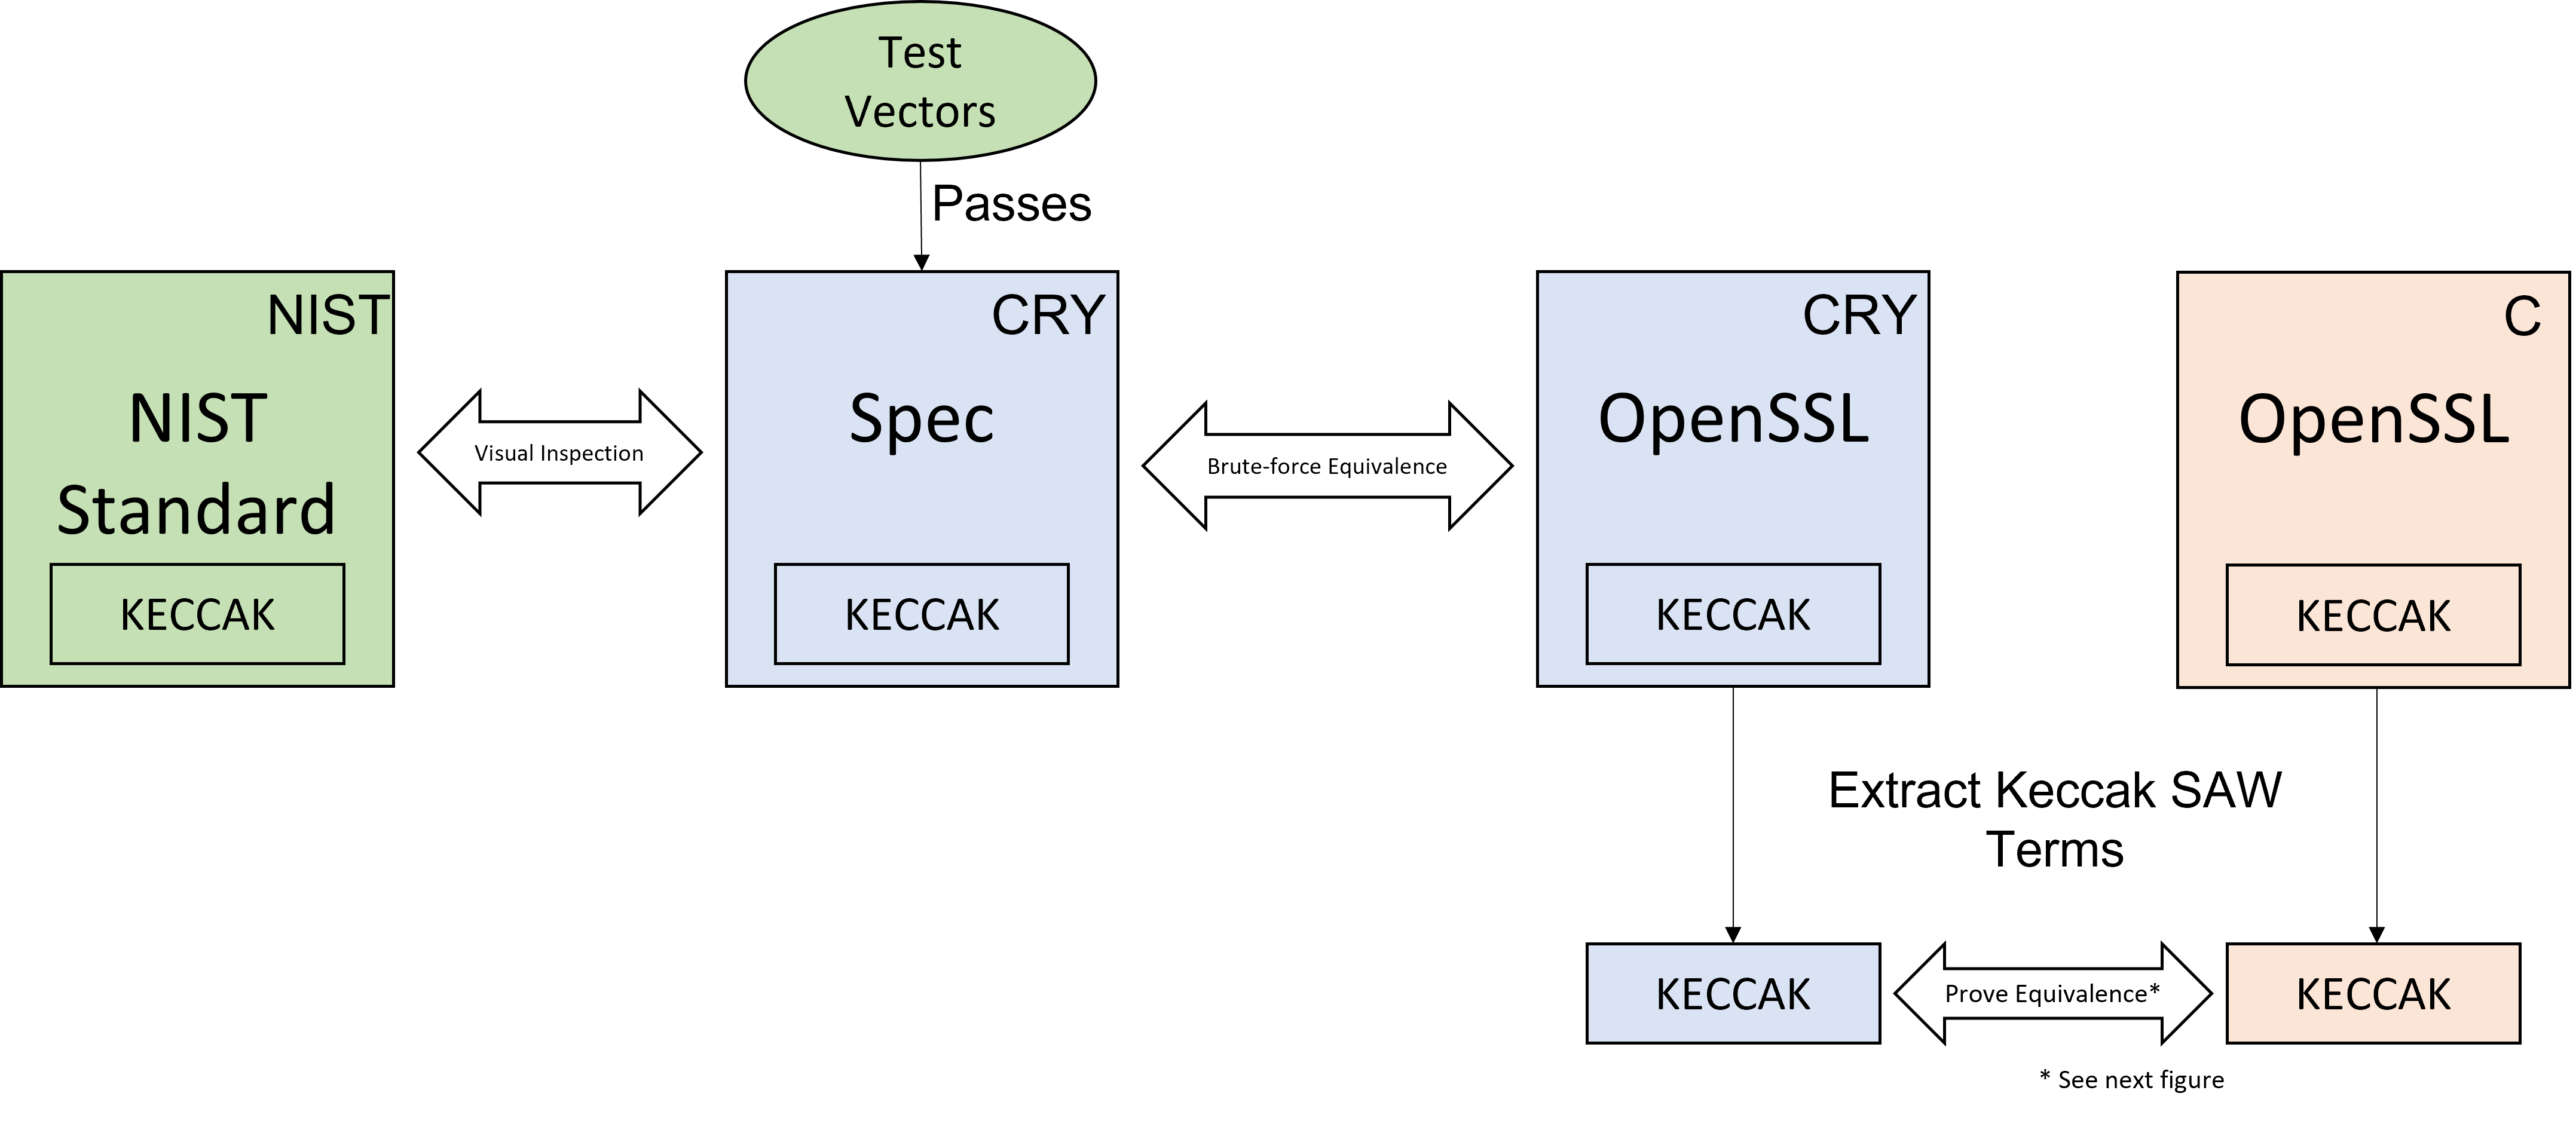
\includegraphics[width=\linewidth]{figs/proof.png}
  
  \caption{SHA3 Keccak Proof Structure}
  \label{fig:proofStructure}
  
\end{figure*}
\begin{figure*}[ht]
  \centering
  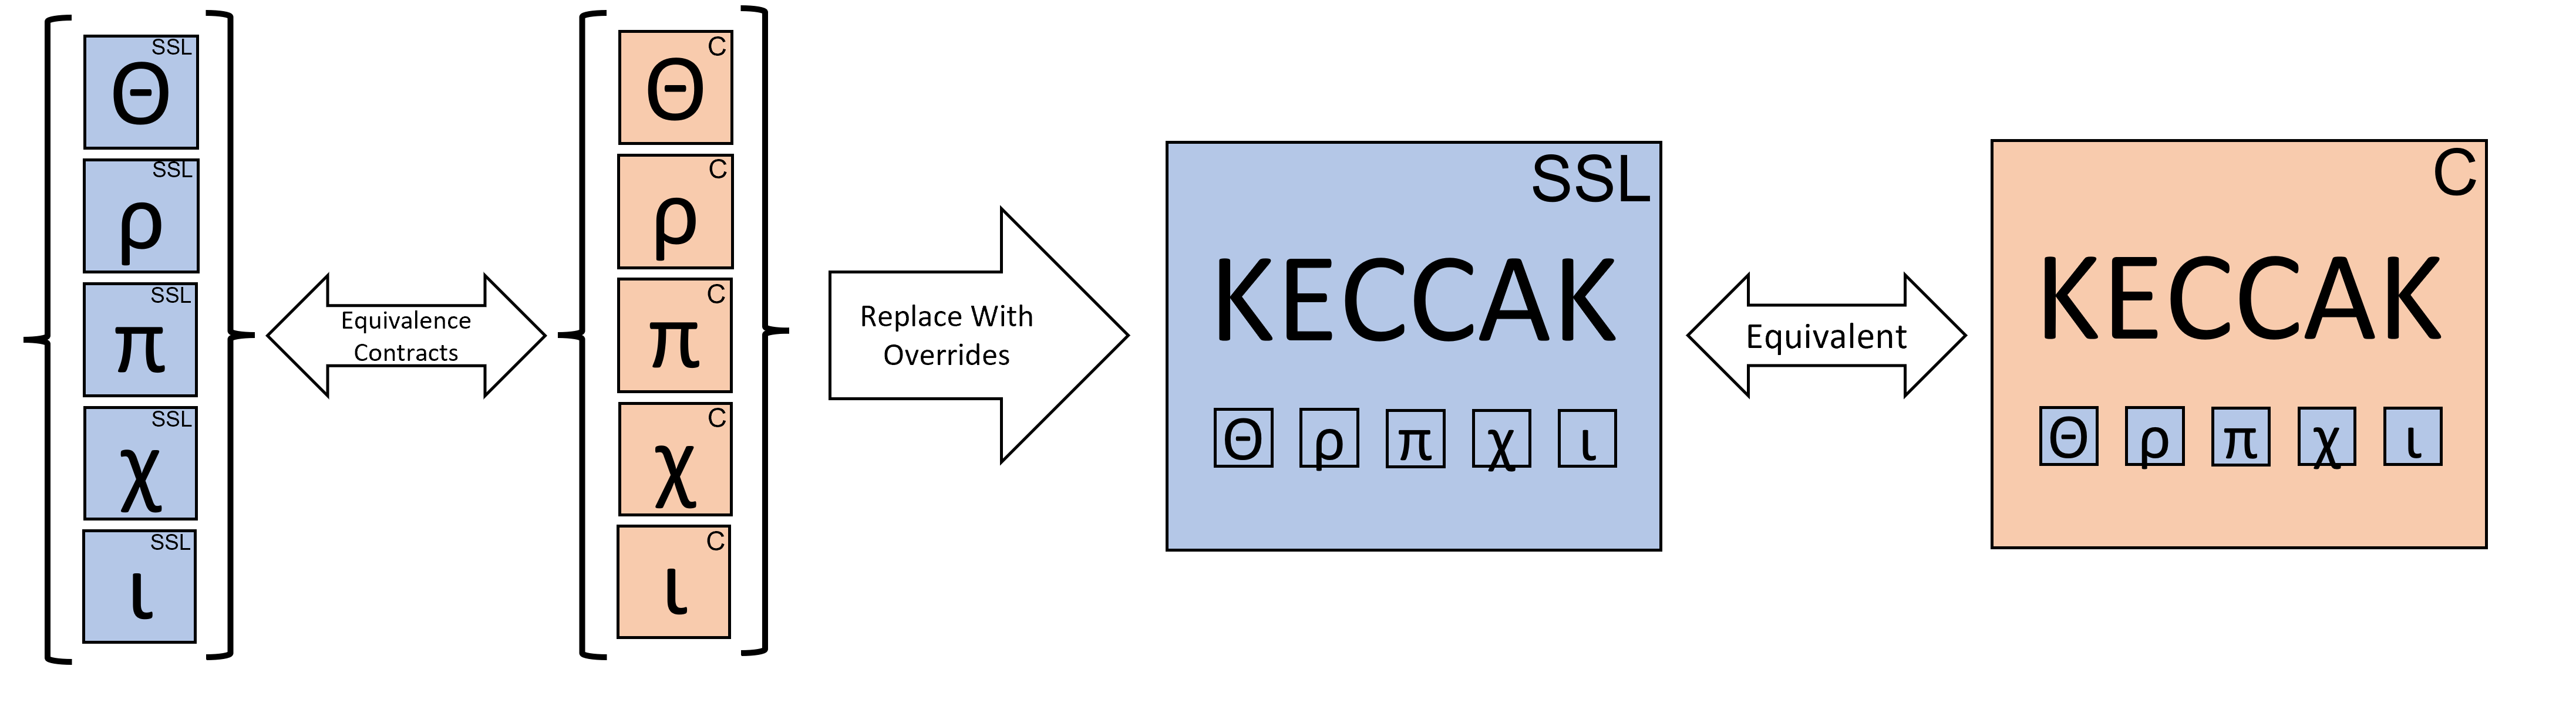
\includegraphics[width=\linewidth]{figs/proof2.png}
  
  \caption{Inner Function Contracts}
  \label{fig:proofStructure2}
  
\end{figure*}

\begin{compactitem}
  \item Process 1600 bits at a time: $5 * 5 * 64$
  \item State vector is $5*5*64*$
  \item Incoming message padded out to whole number of 1600 bit bit-strings
  \item Processed in order by \texttt{KECCAK}
  \item Keccak turns each block into a state vector (rearranges bit layout in memory)
  \item Keccak has 24 rounds for state vector. 
  \item There are 5 hash functions sequentially applied in each round to iteratively update the state vector
  \item After the last round, keccak turns the state vector back into the bit-string./\item The next unprocessed block is \emph{sponged} (e.g., absorbed) into the current bit-string from the latest keccak and the process is repeated 
  \item The digest size is defined in pairs by the standard.
  \item The final bit-string from keccak after sponging and processing every block in the original message is truncated to the desired digest size
  \item The brute force proof is for a digest of 256-bits.
\end{compactitem}

SAW Details


SAW provides a verification environment for compositional proofs of functional equivalence between two pieces of supported code (C, Java, or Cryptol).
SAW uses symbolic execution to create computational models of the code and creates problems of functional equivalence between those two models that can be pushed off to an SMT solver.  
The difficulty of these SMT problems is directly affected by the size and complexity of the computations that are being compared.
This can lead to drastic increases in proof times and sometimes even prevents completion as computations increase.  
SAW's solution to this is to create contracts (called overrides) of a functions input to output relationship which allows for a modular approach to writing the proof.
By breaking up computation into smaller pieces, and creating overrides for these pieces, SAW can often simplify an otherwise complex (and thus incompletable) proof to remain within the capacity of an SMT solver.

Cryptol is a domain-specific specification language, which has been used in the previously mentioned works by Galois' and by Decker et. al to write visually reviewable implementations of NIST standards.
It has strong ties to the SAW tool and, in fact, can be compiled directly down to the SAW Terms (computational models) which are used by SAW in proving functional equivalence.
Because of the interwoven nature of Cryptol with SAW, the Terms created from Cryptol are in most cases significantly simpler than any created through symbolic execution of C/Java code.

The published NIST standards provide no compileable implementation that can be used as a starting point for proving out the algorithm.
As a result, any proof of correctness with a NIST standard is limited in strength to how simple it is use visual review to connect code used in the proof to the NIST standard, coupled with a small sampling of test vectors.
As shown in \ref{proofStructure}, The proof flow starts with a specification of the SHA3 algorithm in Cryptol with the goal of being as similar visually to the NIST standard as possible.
This work discusses significant ways that Cryptol's functional nature can be leveraged to aid in this goal.
Along with simplifying the visual inspection process, this Cryptol specification also passes all test vectors provided by NIST.

The end goal of this proof is to show functional equivalence between this visually reviewable specifications Keccak function, and that of OpenSSL's C code.
Unfortunately, a direct proof between this specification, and OpenSSL's implementation proved unfeasible, because OpenSSL varies from the NIST standard in how it stores the bits of the intermediate state array in memory.
These minor modifications in memory storage put such a proof out of SAW's capabilities, because it relies on strict typing, and comparison of a Cryptol functions input/output to a C functions memory state.
In order to bridge that gap, a second Cryptol specification is included in the proof flow.
It matches in every way the first Cryptol code, except when it comes to how the state array is stored and accessed (at which point it follows OpenSSL's form).
Because of the efficient nature of Cryptol's compilation to SAW Terms, proving equivalence between these Cryptol implementations was possible at the top level of the SHA3 algorithm (which allows for the differences in state array storage to be fully abstracted out).
Due to the strict typing nature required for writing SAW proofs, the scope of this equivalence proof is limited to a given input message size.
The only computations that change in the SHA3 algorithm due to message size are in the padding and sponging of a block.
With this in mind, an exhaustive proof run over each input message byte count from 1 to the block size is sufficient to cover the differences in computation.
The artifact repository accompanying this work contains the receipts of this exhaustive proof. (REFERENCE TO PROOF!!!!)

INNER GREEK FUNCTIONS:

CONTRACTS CAN BE USED TO OVERRIDE AND REPLACE C WITH Cryptol

WITH THESE CONTRACTS SAW CAN COMPLETE A PROOF OF EQUIVALENCE BETWEEN TWO PIECES OF CODE.

This work relies on the correctness of several tools, including language compilers. 

\noindent \textbf{Trusted Code Base}:
\begin{itemize}
  \item LLVM bitcode compiler
  \item The Software Analysis Workbench (SAW) including the conversion from LLVM bitcode to SAWCore terms, the Cryptol compiler to SAWCore terms, and SAW's interface with SMT solvers.
  \item The z3, abc, and yices SMT solvers.
\end{itemize}

Talk about the cost of the verification. The amount of effort required to write the specification. Make clear the limits of the result proof.

\begin{compactitem}
\item Visual inspection and limited test vectors for (1) and (2)
\item Only provide proof certificates for message sizes of X to Y for digest sizes of \textbf{FIXME} for (3)
\item Visual inspection only for anything above Keccak for (3) in OpenSSLs C-code
\end{compactitem}

Effort (see above and then consider below):
\begin{compactitem}
 \item How long were we working on the Cryptol code?
 \item How long were we working on the SAW proofs?
 \item How long did it take to understand the OpenSSL code?
\end{compactitem}
We'll want to determine how long it took us and then try to infer how long that would have taken had we been working full time (40 hours/week).

Because of the modular design of the SHA-3 specification, the Cryptol implementation and OpenSSL implementation are programmatically more similar. 
The only strong discrepancy is that the OpenSSL implementation organizes the bits of the sponge construction. 
The affect of modular cryptographic design can be seen by the proof completing successfully in the Yices, Z3, and ABC SMT-solvers. 
Previous work on SHA2-256 was only successful with Yices \cite{nfm-us}. Full results are show in table \ref{finaltable}. 

\begin{table*}[b]
\caption{Proof Runtimes for SHA-3 with SMT-solvers}\label{finaltable}
\setlength{\tabcolsep}{13.5pt}
\begin{tabular}{|l|r|r|r|}
\hline
\textbf{Function} & \textbf{Yices} & \textbf{Z3} & \textbf{ABC} \\
\hline
Pi          &   0.895 secs &    11.072 secs &    0.417 secs \\
Rho         &   4.509 secs &    15.776 secs &    5.879 secs \\
Theta       &  25.942 secs &    11.345 secs &   14.869 secs \\
Chi         &   5.059 secs &     3.930 secs &    1.327 secs \\
Iota        &  11.048 secs &     8.801 secs &  612.497 secs \\
KeccakF1600 & 745.206 secs & 15187.671 secs & 2910.549 secs \\
\hline
\end{tabular}
\end{table*}
